\chapter{Sheaf Pitches}

\newthought{Sheaves} are a tool to integrate local data into one global state.
In sheaf terminology, certain combinations of local sections correspond to a
global section. Defining a sheaf therefore necessitates defining a set of local
sections and a method of consistent integration. There are two different
decompositions of images into local sections that I'm considering: expert
knowledge decomposition and geometric decomposition.

\section{Expert Knowledge Decomposition}

\newthought{The intuition} behind expert knowledge decomposition is that
several experts will fill in gaps in knowledge left by others. Each expert is a
local section, and, when all of their opinions are composed, the final image
(or a labeled final image?)  that is consistent between all experts is
(re)generated.

\newcommand{\yslant}{0.5}
\newcommand{\xslant}{-0.6}
\begin{marginfigure}
\begin{tikzpicture}[scale=1.1,every node/.style={minimum size=1cm},on grid]
	\begin{scope}[
		every node/.append style={yslant=\yslant,xslant=\xslant},
		yslant=\yslant,xslant=\xslant
	] 
		% The frame:
		\draw[black, dashed, thin] (0,0) rectangle (2.5,2); 
		\node [anchor=south west](expertP) at (0,0)
		{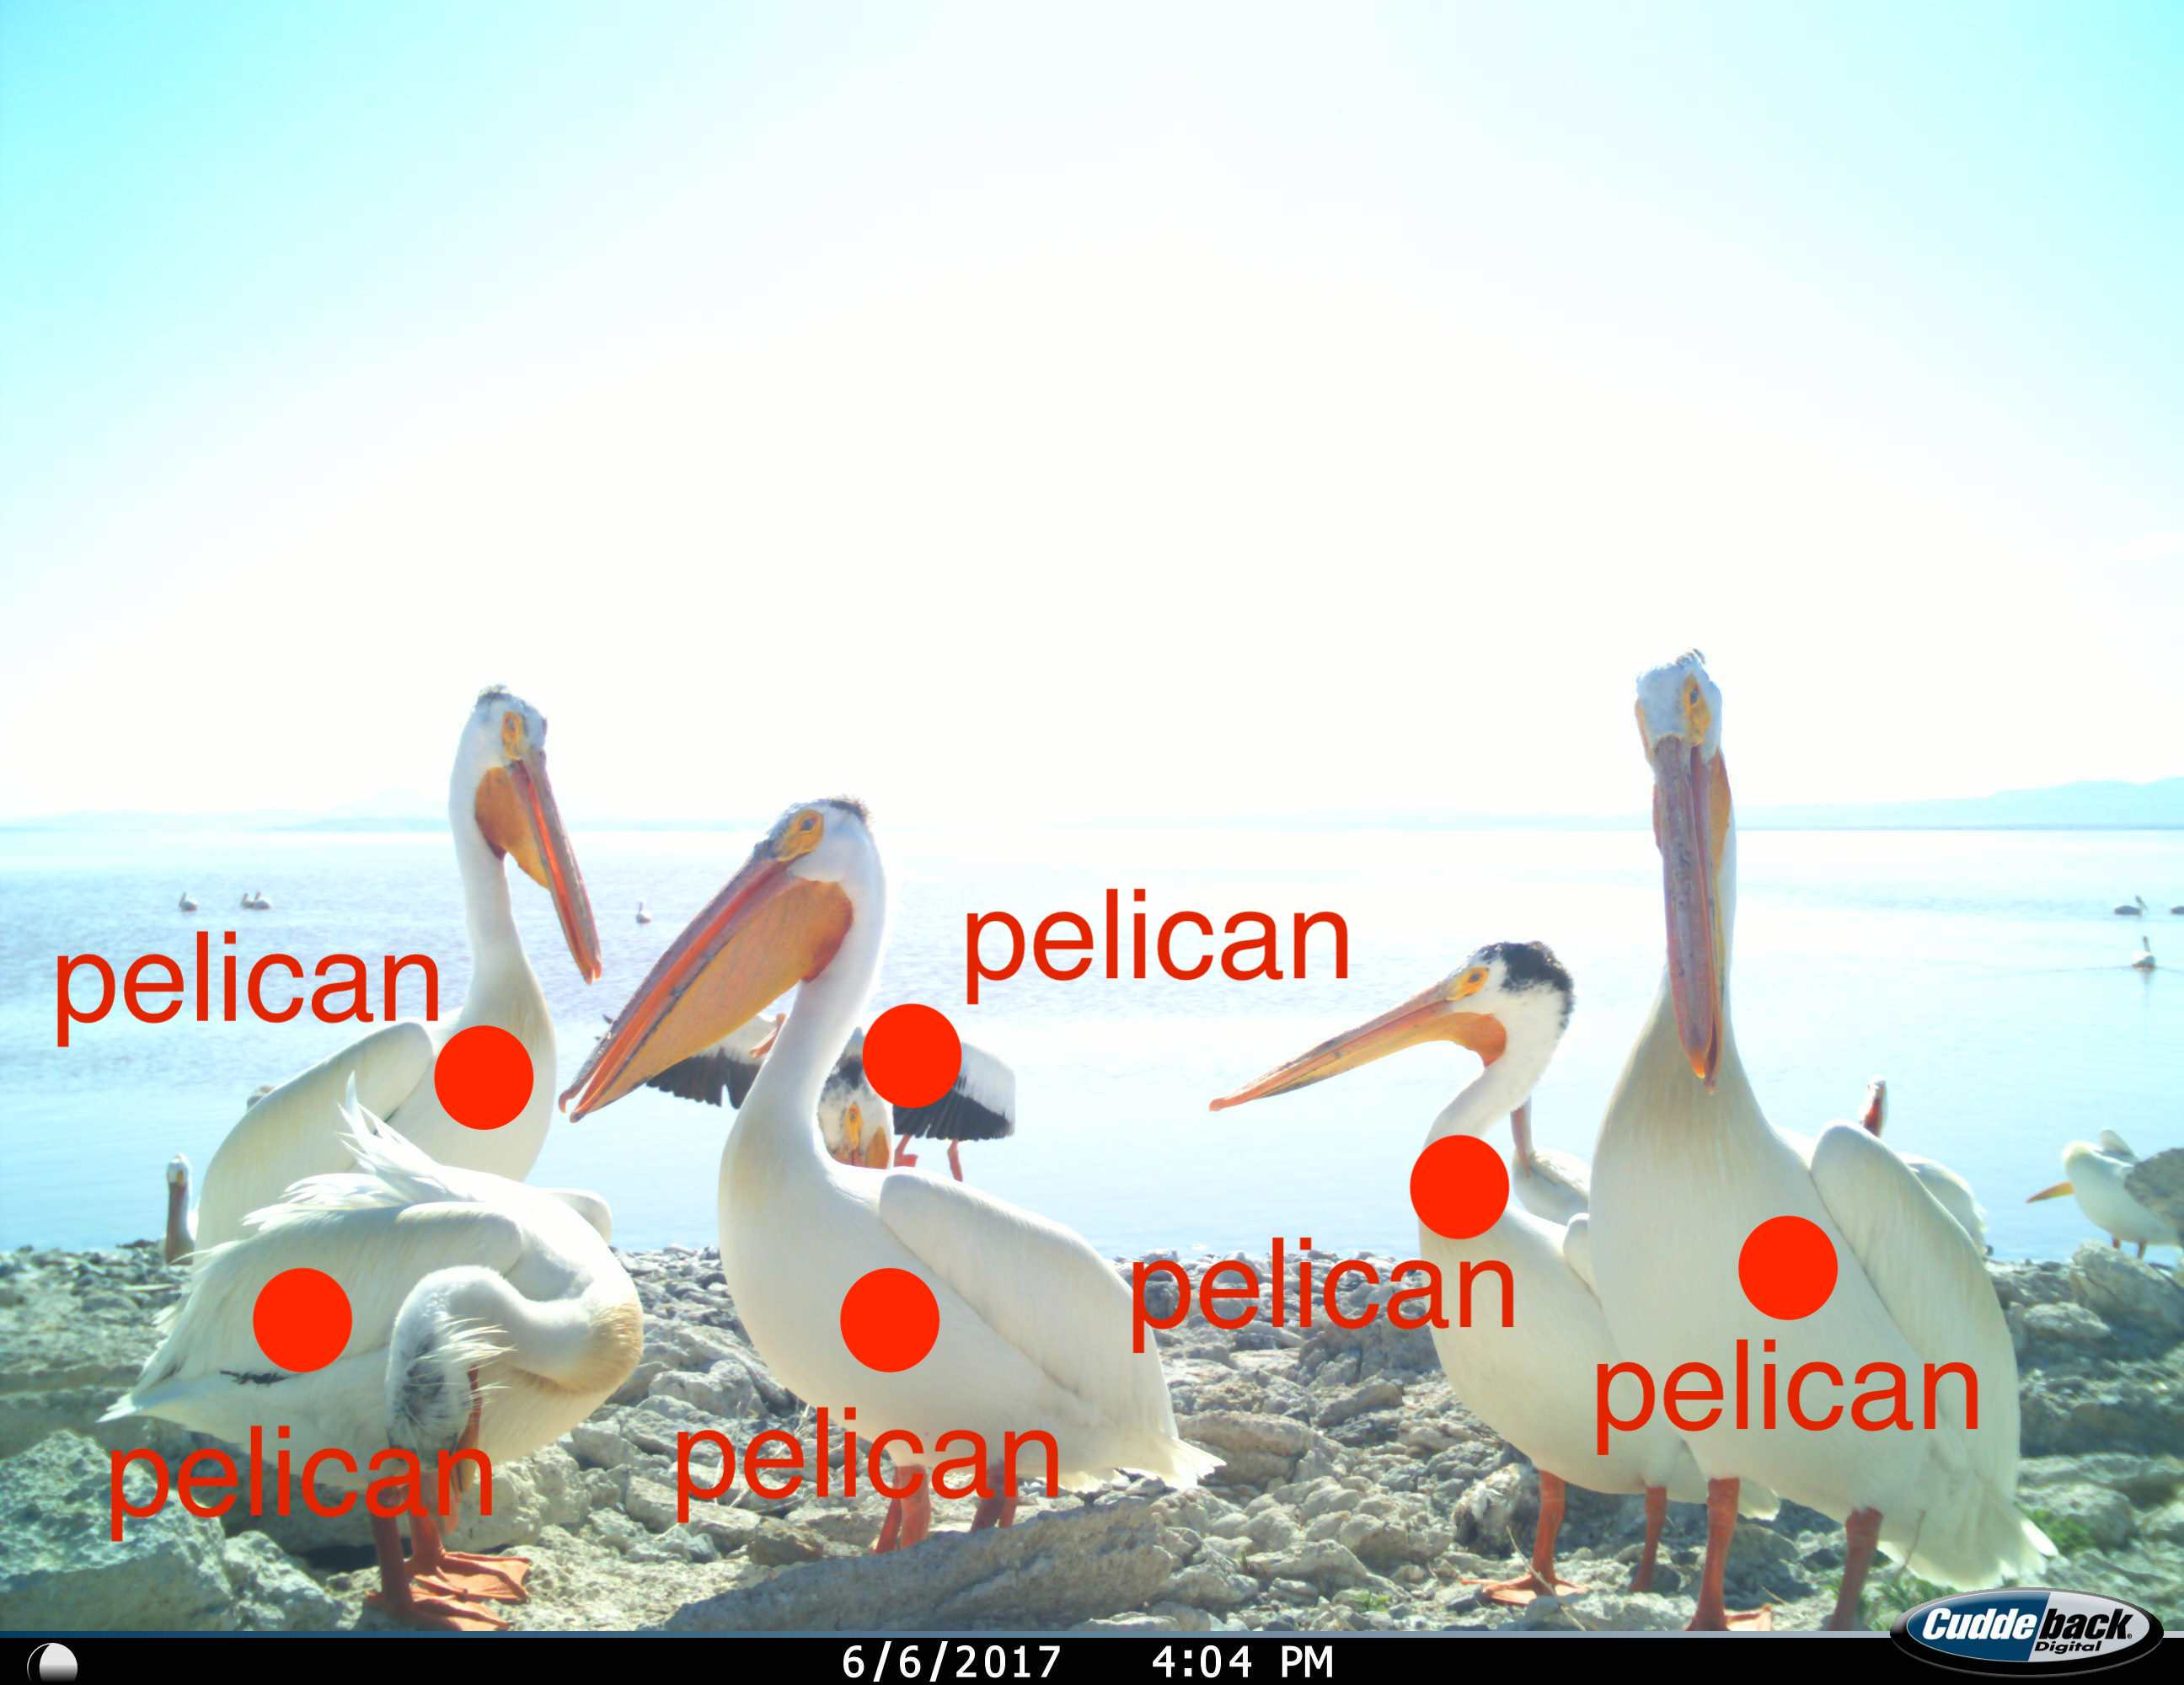
\includegraphics[width=0.5\linewidth]{img/pelicansEp.jpg}};
		\draw[black, dashed, thin] (2.6,0) rectangle (5.1,2); 
		\node[anchor=south west](expertT) at (2.6,0)
		{
\includegraphics[width=0.5\linewidth]{img/pelicansEt.jpg}};
	\end{scope}
	\begin{scope}[
		yshift=-80,
		every node/.append style={yslant=\yslant,xslant=\xslant},
		yslant=\yslant,xslant=\xslant
	] 
		% The frame:
		\draw[black, dashed, thin] (1.1,0) rectangle (3.6,2); 
		\node[anchor=south west] (both) at
		(1.1,0){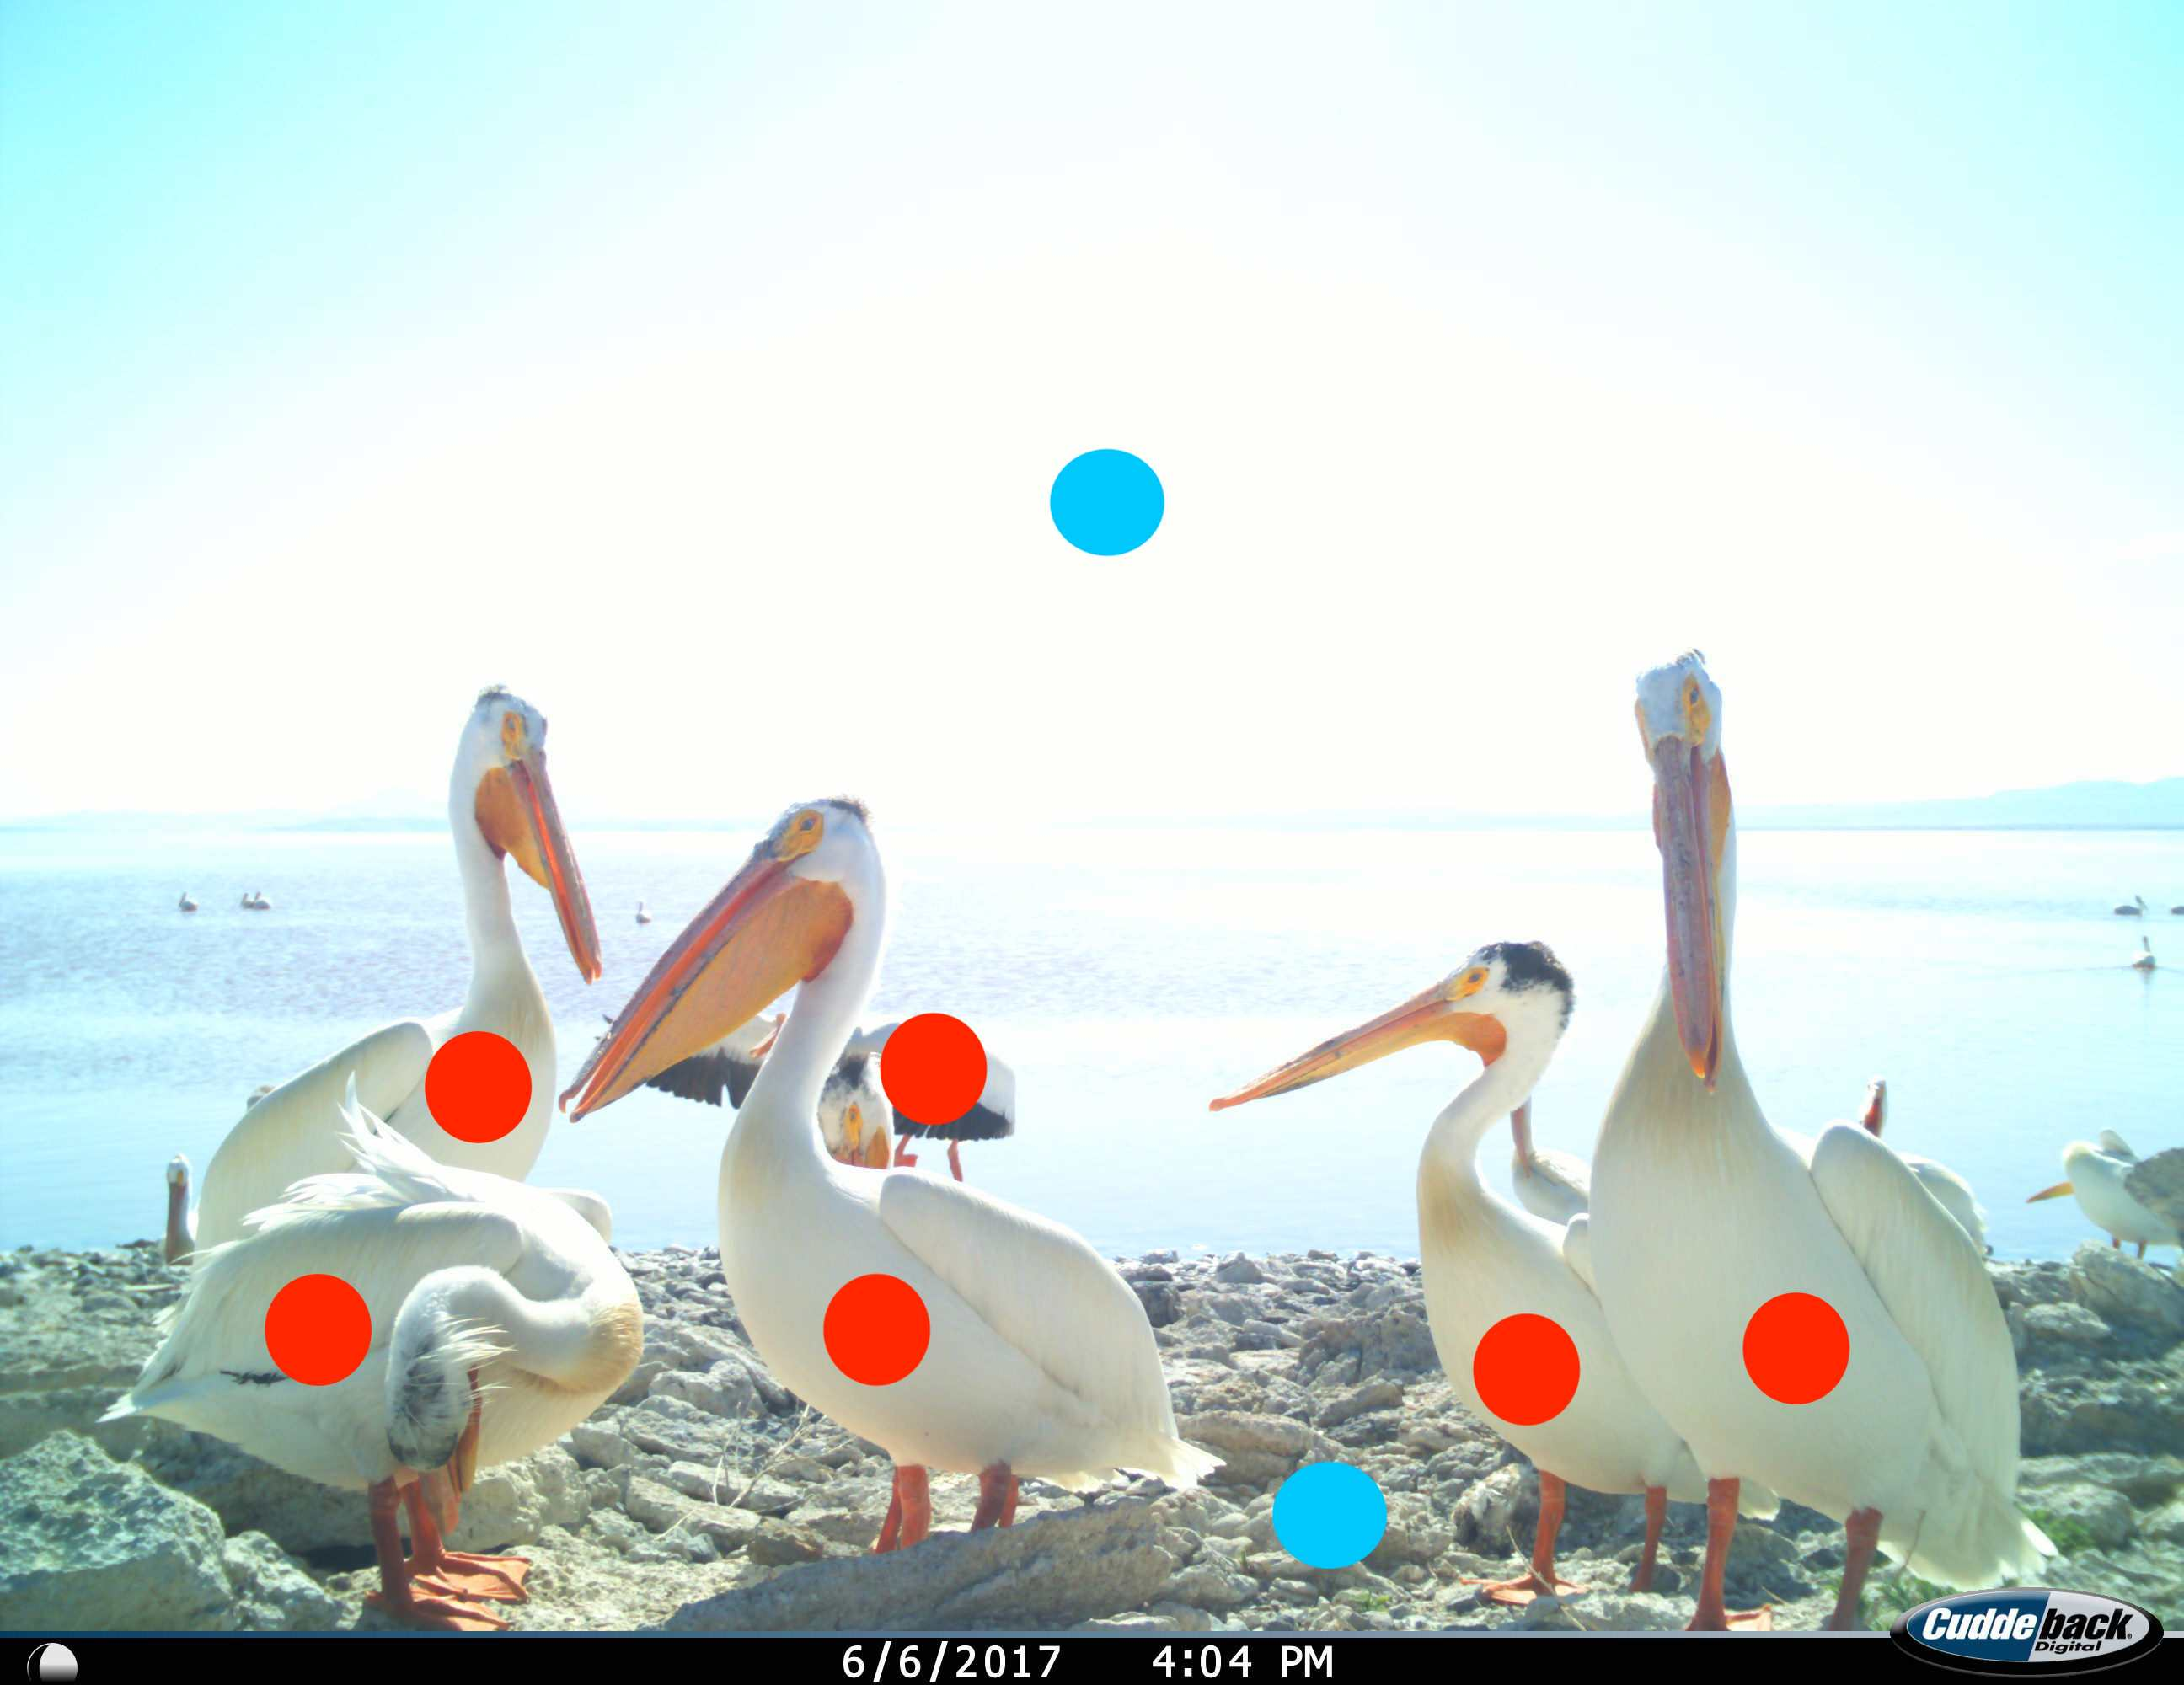
\includegraphics[width=0.5\linewidth]{img/pelicansB.jpg}};
	\end{scope}
	\draw (expertT) -- node[near end, left] {merge} (both) ; 
	\draw (expertP) -- (both) ; 
\end{tikzpicture}
\end{marginfigure}

An intuitive example can be thought of by having two experts: a topographic
expert and a pelican expert. The topographic expert has learned to recognize
the beach, and can match parts of the image to a 3D model of the beach. The
pelican expert is trained identify potential pelicans. So, it can recognize
likely pods, etc. The insight is this: there are parts of the image that are
not the beach. The topographic expert will therefore have gaps in the image
that it might consider \emph{not part of the beach}. Integrating the opinion of
both experts would generate a labeled version of the image, with each pixel
assignable to either a pelican or the beach. The importance is the consistency
between experts. If the beach expert strongly believes that there are parts of
the beach that the pelican expert weakly believes are pelicans, then pelicans
will not be identified there. The experts must fill in the gaps left by other
experts.


A relevant question is, if the pelican expert exists, isn't that really all
that's needed for the project? What is the point of the other experts? There
are two reasons I can think of to have multiple experts, 1) a pelican expert
will trained to detect pelicans will have a pelican bias and 2) training a
pelican expert might not be feasible or what we want. It would be easier to
train an expert on pelican pods, pelicans in flight, closeup pelicans, faraway
pelicans, and have these experts all render an opinion.

So what would the integration look like? In the two-expert example, integration
would be merging the two sets of labels. Each pixel can be assigned a
\emph{pelican} label by the pelican expert or a \emph{beach} label by the
topography expert. Integration is successful if pixels do not receive the same
label. Notice that disjoint labeling makes sense in this case; however, two
experts trained to identify the same class of object (e.g. an expert in pelican
pods and an expert in identifying birds) should assign the same label to the
same pixel rather than avoid labeling the same pixel.

\section{Geometric Decomposition}

\newthought{Geometric decomposition} is a little ``flatter'' in that the labels
are all rendered at the same time, and the integration is where evidence is
strengthened or weakened. An intuitive example comes from decomposing the image
into 2D squares, and stiching these into larger and larger regions. Considering
the edge of the square, we can see how experts may interact. It may be that a
pelican is split between two quadrants. The integration of the two quadrants
requires that they both agree on the pelican on their boundary, and, possibly
on knowledge more specific than that. For example, if the bill is on one
quadrant, that quadrant must expect the body to be on its adjacent quadrant.
The integration step then considers stitching the boundaries by having experts
all examine adjacent quadrants and setting labels to the edges. The labels on
these edges, or more generally, the labels that one quadrant predicts for its
adjacent quadrants are matched during the integration phase.

One of the open questions is whether all experts will be active on each
quadrant or not. If we have a pelican pod expert, there is a chance that a
positive reading on a pod will not be achievable until multiple quadrants have
been merged.


